Alla luce delle funzionalità che gli emulatori di rete oggi esistenti offrono, desideriamo, con l'obiettivo di approfondire le nostre conoscenze in ambito di reti e di sviluppo software, proporre una soluzione alternativa che offra feature extra ed un miglioramento generale della qualità di utilizzo.
\subsection{Funzionalità}
Le funzionalità che desideriamo offrire attraverso l'utilizzo di \texttt{DONE} sono le seguenti: 
\begin{itemize}
    \item L'utente può creare, aprire, modificare \textbf{progetti di topologie di rete}, aggiungendo apparati, definendo collegamenti tra questi, nonché fare uso di device specifici volti al collegamento della topologia definita a reti esterne alla simulazione. I dispositivi utilizzabili sono hub, switch, nodi, router, connessioni a interfacce esterne, con NAT o meno.
    \item Una volta realizzata la topologia desiderata, l'utente può \textbf{salvare su file il progetto}, con lo scopo di poter riprendere il lavoro in un secondo momento.
    \item L'utente può assegnare per ogni singolo device delle \textbf{configurazioni} che verranno applicate all'avvio della simulazione.
    \item L'utente può avviare la simulazione, con la possibilità in seguito di \textbf{accedere tramite terminale ai singoli nodi} per aggiungere ulteriori configurazioni, per testare la connettività e/o effettuare troubleshooting. Il tutto esclusivamente tramite linea di comando. I nodi possono ospitare vari servizi, come ad esempio server ssh, ftp e web, anch'essi configurabili da linea di comando. 
\end{itemize}
Gli obiettivi che desideriamo perseguire con questo progetto sono:
\begin{itemize}
    \item \textbf{Ridurre le dipendenze} al minimo necessario, in modo da rendere il programma il più portabile possibile.
    \item Fornire la \textbf{capacità di salvare} non solo la topologia fisica, ma anche tutte le configurazioni, senza bisogno di script ulteriori.
    \item \textbf{Maggiore pulizia dell'ambiente}, evitando che Docker rimanga in uno stato intermedio (ossia con i vecchi container ancora presenti) in caso di chiusura della applicazione senza arresto della simulazione, nonché pulizia dalle altre interfacce e apparati virtuali creati.
    \item Offrire una soluzione open-source che possa essere \textbf{estesa} e \textbf{modificata}.
\end{itemize}
\subsection{Architettura}
Alla luce delle funzionalità desiderate, l'architettura che abbiamo ideato per raggiungere gli obiettivi preposti è così organizzata: 
\begin{center}
    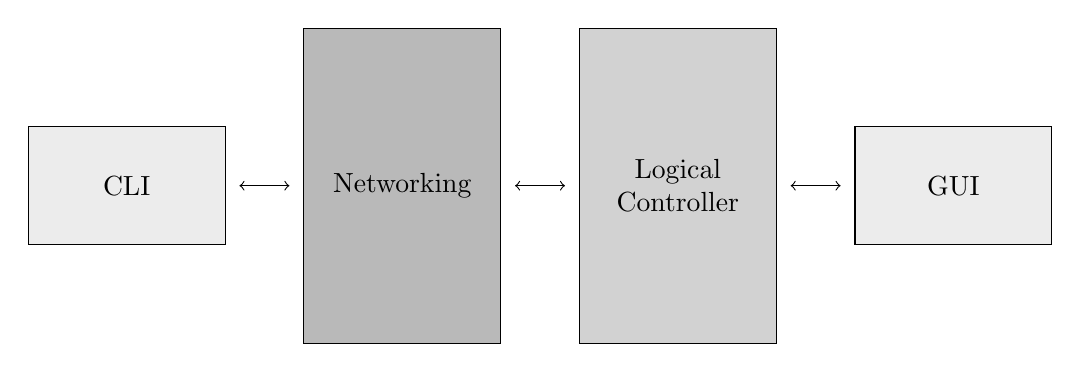
\begin{tikzpicture}
        \node[rectangle,draw,minimum height=4cm,minimum width=2.5cm,align=center,fill=gray!55] (net) at (-2.5,0) {Networking};
        \node[rectangle,draw,minimum height=4cm,minimum width=2.5cm,fill=gray!35,align=center] (log) at (1,0) {Logical\\Controller};
        \node[rectangle,draw,minimum height=1.5cm, minimum width=2.5cm,fill=gray!15] (gui) at (4.5,0) {GUI};
        \node[rectangle,draw,minimum height=1.5cm, minimum width=2.5cm,fill=gray!15] (cli) at (-6,0) {CLI};
        \draw[<->, shorten >= 5pt, shorten <= 5pt] (net) -- (log);
        \draw[<->, shorten >= 5pt, shorten <= 5pt] (log) -- (gui);
        \draw[<->, shorten >= 5pt, shorten <= 5pt] (net) to (cli);
    \end{tikzpicture}
\end{center}
Pertanto, le componenti da realizzare sono:
\begin{itemize}
    \item \textbf{Networking}: Utilizzo di container e apparati virtualizzati. Si tratta del modo in cui vengono realizzati, come in IMUNES, i componenti veri e propri. Essi sono poi connessi tra di loro mediante gli appositi comandi e possono simulare una rete. Sarà gestito dal relativo controller attraverso librerie apposite sviluppate ad hoc.
    \item \textbf{Logical Controller}: Automatizzazione, a fronte di una topologia creata, della creazione della configurazione di rete e realizzazione di logica di controllo, a più alto livello, che possa gestire:
          \begin{itemize}
              \item Strutture relative alla topologia creata;
              \item Salvataggio della topologia;
              \item Gestione e salvataggio delle configurazioni;
              \item Invio delle informazioni necessarie al livello di Networking per generare la topologia creata.
          \end{itemize}
    \item \textbf{GUI}: si tratta dell'interfaccia su cui l'utente può disegnare la topologia logica della rete, posizionando quindi nodi e link tra nodi, rilocandoli, modificandoli e interagendoci.
    Permetterà di accedere a CLI dedicate ai singoli nodi per inserire configurazioni.
    \item \textbf{CLI}: offre un'alternativa all'utilizzo combinato di GUI e logical controller, permettendo di interagire direttamente col livello di networking\footnote{I due approcci sono mutualmente esclusivi: scegliere di utilizzare la CLI in fase di progettazione significa rinunciare alla possibilità di salvare la configurazione e la disposizione dei nodi che sono invece parte integrante dell'approccio predefinito GUI - Logical Controller.}. Essa consiste in un'istanza interattiva di Python arricchita da funzioni ad hoc che consentono di modificare il sistema live fin dalla fase di progettazione.
\end{itemize}
È inoltre prevista la possibilità, durante la simulazione, indipendentemente dalla scelta della modalità di utilizzo (sia essa GUI o CLI), di connettersi tramite \textbf{shell} ai singoli nodi.



\newpage
